\documentclass[10pt,a4paper]{article}

\renewcommand*\rmdefault{ppl}

\usepackage[utf8]{inputenc}
\usepackage[T1]{fontenc}
\usepackage[english]{babel}                 % Anpassung f\"ur deutsche Sprache
\usepackage{amsmath}
\usepackage{graphicx}
\usepackage{caption}
\usepackage{subcaption}
\usepackage{listings}
\usepackage{algorithm,algorithmic}
\usepackage{a4wide}
\usepackage{bm}

\newtheorem{theorem}{Theorem}[section]
\newtheorem{lemma}[theorem]{Lemma}
\newtheorem{proposition}[theorem]{Proposition}
\newtheorem{corollary}[theorem]{Corollary}

\usepackage{amssymb}

\newenvironment{proof}[1][Proof]{\begin{trivlist}
\item[\hskip \labelsep {\bfseries #1}]}{\end{trivlist}}
\newenvironment{definition}[1][Definition]{\begin{trivlist}
\item[\hskip \labelsep {\bfseries #1}]}{\end{trivlist}}
\newenvironment{example}[1][Example]{\begin{trivlist}
\item[\hskip \labelsep {\bfseries #1}]}{\end{trivlist}}
\newenvironment{remark}[1][Remark]{\begin{trivlist}
\item[\hskip \labelsep {\bfseries #1}]}{\end{trivlist}}
\DeclareMathOperator*{\argmin}{arg\,min}

\newcommand{\qed}{\hfill \ensuremath{\Box}}
\setlength{\parindent}{0pt}

\raggedbottom

\begin{document}
\section*{Multilevel S$_N$ for applications in radiation therapy}
The idea of this project is to implement an efficient, but readable S$_N$ code framework. Such a code framework can be used for different applications and we wish to first use it for problems in radiation therapy. Furthermore, we can use the framework to test the idea of multilevel S$_N$, which splits the spatial domain into grids with varying resolution and uses a fine quadrature set on coarse grids as well as coarse quadratures on fine grids\footnote{One could also think about going one step further by extending the multilevel idea to uncertainty quantification for multilevel S$_N$.}. Two main working "products" could be papers on \textit{S$_N$ for radiation therapy}, \textit{Multilevel S$_N$}, \textit{Effects of quadrature sets and triangular discretizations} as well as a functioning and documented software. In the following, we briefly mention the fundamentals of the S$_N$ method and state the idea of multilevel S$_N$:

\section{The discrete ordinates (S$_N$) method}
The radiative transfer (or linear Boltzmann) equation reads
\begin{align}\label{eq:radTransfer}
\partial_t \psi(t,\bm x,\bm\Omega) + \bm\Omega\cdot\nabla \psi(t,\bm x,\bm\Omega) + \sigma_a(\bm x)\psi(t,\bm x,\bm\Omega) = \sigma_s(\bm x) \int_{\mathbb{S}^2} k(\bm\Omega\cdot\bm\Omega')\left(\psi(t,\bm x,\bm\Omega')-\psi(t,\bm x,\bm\Omega)\right)\,d\bm\Omega'.
\end{align}
The equation describes the dynamics of particles traveling through a background material. Particles are subject to absorption (described by the absorption cross section $\sigma_a$) as well as scattering (described by the scattering cross section $\sigma_s$ as well as the collision kernel $k$). Note that for now, we omit the effects of sources. Also, when following the work of Kerstin \cite{kupper2016models}, one often solves the continuous slowing down (CSD) equation for treatment planning, which is closely related to the radiative transfer equation. Hence, a starting point for obtaining a working code base could be \eqref{eq:radTransfer}.

In the field of radiation therapy, the radiative transfer equation is often discretized by Monte-Carlo methods, which commonly yield an increased runtime and stochastic noise. Therefore, we choose a discrete ordinates (S$_N$) discretization (which has its own disadvantages such as ray-effects) instead. The first step to obtain a discretized system is to derive a finite dimensional, nodal representation of the angular variable $\bm\Omega\in\mathbb{S}^2$. Here, different strategies to obtain an accurate discretization exist and we are going to start with a straight forward product quadrature rule on the sphere. To obtain a finite set of directions in $\mathbb{S}^2$, we describe the angular variable
\begin{align*}
\bm\Omega = (\cos\phi \sin \theta, \sin\phi \sin \theta, \cos \theta)^T\;
\end{align*}
at finite positions of $\theta$ and $\phi$. In the following, we choose the nodal positions of $\mu = \cos(\theta) \in[-1,1]$ to be the quadrature points of a Gauss quadrature rule with $N_q$ quadrature points, while choosing an equally spaced grid for $\phi$, i.e.
\begin{align*}
\phi_i = i \Delta\phi \quad \text{for} \quad i=1,\ldots,N_q \quad \text{and} 
\quad \Delta\phi = \frac{2\pi}{N_q}\;.
\end{align*}
Now, we have a finite number of nodal directions (also called ordinates) on the sphere, which we denote by $\Omega_k$ for $k = 1,\cdots, Q$, where $Q:=N_q^2$. The solution at these ordinates is defined as $\psi_p(t,\bm x):=\psi(t,\bm x,\bm\Omega_p)$. Furthermore, one can construct a quadrature rule
\begin{align*}
\int_{\mathbb{S}^2} \psi(t,\bm x,\bm\Omega)\,d\bm\Omega \approx \sum_{q=1}^Q w_q \psi_q(t,\bm x).
\end{align*}
Now, evaluating the radiative transfer equation \eqref{eq:radTransfer} at the chosen set of ordinates while making use of the above quadrature rule yields
\begin{align*}
\partial_t \psi_p(t,\bm x) + \bm\Omega_p\cdot\nabla \psi_p(t,\bm x) + \sigma_a(\bm x)\psi_p(t,\bm x) = \sigma_s(\bm x) \sum_{q=1}^Q w_q k(\bm\Omega_p\cdot\bm\Omega_q)\left(\psi_q(t,\bm x)-\psi_p(t,\bm x)\right).
\end{align*}
This is now a system of $Q$ advection equations with a coupling term on the right hand side. Such an equation can be solved in a straight forward manner with a finite volume discretization (we could also think about using DG). For this, we split the (for now two-dimensional) spatial domain into cells $V_{ij} = [x_{i-1/2},x_{i+1/2}]\times[y_{j-1/2},y_{j+1/2}]$ and describe the time evolution of the solution on these cells. Let us denote the solution in cell $V_{ij}$ at time $t_n$ as
\begin{align*}
\psi_{pij}^n := \frac{1}{\vert V_{ij}\vert}\int_{V_{ij}} \psi_p(t_n,\bm x)\,d\bm x.
\end{align*}
At time $t_0 = 0$, the initial particle density is known. To obtain a scheme which time updates the solution, we (when leaving out certain details) replace the time derivative by a finite difference approximation
\begin{align*}
\partial_t \psi_p(t,\bm x_{ij})\Big\vert_{t = t_n} &\approx \frac{\psi_{pij}^n-\psi_{pij}^n}{\Delta t}\;, \\
(\bm\Omega_p)_x\partial_x \psi_p(t^n,\bm x)\Big\vert_{\bm x = \bm x_{ij}} &\approx \frac{1}{|V_{ij}|} \left( g_{p,i+1/2,j}^n - g_{p,i-1/2,j}^n \right)\;, \\
(\bm\Omega_p)_y\partial_y \psi_p(t^n,\bm x)\Big\vert_{\bm x = \bm x_{ij}} &\approx \frac{1}{|V_{ij}|} \left( g_{p,i,j+1/2}^n - g_{p,i,j-1/2}^n \right)\;.
\end{align*}
The function $g_{p,i+1/2,j}$ is called the numerical flux, which approximates the solution at the cell interface at $x_{i+1/2}$. One straight forward choice is the upwind flux
\begin{align*}
g_{p,i+1/2,j} := 
\begin{cases}
(\bm\Omega_p)_x \psi_{pij}^{n} & \text{ if }(\bm\Omega_p)_x>0\\
(\bm\Omega_p)_x \psi_{p,i+1,j}^{n} & \text{ else}
\end{cases}\;.
\end{align*}
When replacing differential operators by these approximations, we obtain the first-order scheme
\begin{align}\label{eq:FV}
\psi_{pij}^{n+1} =& \psi_{pij}^{n} - \frac{\Delta t}{\vert V_{ij} \vert} \left( g_{p,i+1/2,j} - g_{p,i-1/2,j} + g_{p,i,j+1/2}- g_{p,i,j-1/2} \right)\nonumber \\
&+\Delta t  \sigma_{s,ij}\sum_{q=1}^{N_q} w_q k(\bm\Omega_p\cdot\bm\Omega_q) \left(\psi_{q,ij}^{n}-\psi_{p,ij}^{n}\right)-\Delta t\sigma_{a,ij} \psi_{pij}^{n}\;.
\end{align}
This is the equation which needs to be implemented. It can be extended to higher order, but we should start with order one.

\section{Physical model}

\section{Multilevel S$_N$}
In the following, we wish to apply ideas from multilevel Monte-Carlo as well as multilevel stochastic-Collocation to the S$_N$ context. Usually, one is not interested in the angular flux $\psi$, but one rather wishes to determine some quantity of interest, which could for example be the radiation dose received by the patient or the angular flux in a certain region. Let us call this scalar quantity $d$, where the bracket denotes a spherical integration and $d:\mathbb{S}^2\rightarrow\mathbb{R}$. We assume a quantity constant in time and space for sake of simplicity. Assume that we can approximate the quantity $d$ with our code using a certain spatial resolution $h:=\Delta x = \Delta y$ as well as $Q$ quadrature points. Then, when the output for resolution $h$ and $Q$ is denoted as $\tilde d^{h,Q}_k$ for $k = 1,\cdots,Q$. This output can be interpreted as a continuous grid function\footnote{A more elegant interpretation is possible when using a spherical harmonics reconstruction or a grid-based quadrature like the octahedron or icosahedron quadrature.}
\begin{align*}
d_{h,Q}(\Omega) := \tilde d^{h,Q}_k \quad \text{ with $k$ s.t. $\Omega_k$ is the closest ordinate to }\Omega.
\end{align*}
Now the L$^2$ distance to the exact quantity of interest $d$ can be divided into an quadrature as well as a spatial error. Adding and subtracting the term $d_{h}$ inside the brackets, where $d_h:\mathbb{S}^2\rightarrow\mathbb{R}$ uses an exact quadrature with a fixed spatial resolution $h$ (i.e. $Q\rightarrow\infty$) yields
\begin{align*}
\Vert d_{h,Q} - d \Vert_{L^{2}(\mathbb{S}^2)} \leq \Vert d_{h,Q} - d_{h} \Vert_{L^{2}(\mathbb{S}^2)}+\Vert d_{h} - d \Vert_{L^{2}(\mathbb{S}^2)}.
\end{align*}
Then, the first term is the quadrature error and the second term is the spatial discretization error. Assume that the following error estimates hold:
\begin{align*}
\Vert d_{h} - d \Vert_{L^{2}(\mathbb{S}^2)} &\lesssim h^{\alpha} \simeq N_x^{-\alpha} \\
\Vert d_{h,Q} - d_{h} \Vert_{L^{2}(\mathbb{S}^2)} &\lesssim Q^{-\beta}.
\end{align*}
A certain accuracy $\varepsilon$ can be obtained by bounding both error terms by $\varepsilon/2$, i.e. the number of spatial cells must be
\begin{align*}
N_x^{-\alpha} \simeq \varepsilon \quad \Rightarrow \quad N_x \simeq \varepsilon^{-1/\alpha}
\end{align*}
and the number of quadrature points has to be 
\begin{align*}
Q^{-\beta} \simeq \varepsilon \quad \Rightarrow \quad Q \simeq \varepsilon^{-1/\beta}
\end{align*}
Assume the cost to run a simulation are $C = N_x^3 \cdot Q$. Then we get
\begin{align}\label{eq:costsMC}
C \simeq \varepsilon^{-\frac{3}{\alpha} - \frac{1}{\beta}}.
\end{align} 
Now let us make a multilevel ansatz. For this we define $L$ levels for the spatial grid resolution $h_{\ell}$ with $\ell = 1,\cdots,L$. Then, we can write $d_{h_L,Q}(\Omega)$, i.e. the quantity of interest for the finest resolution $h_L$ with a certain number of quadrature points as
\begin{align}\label{eq:MLSNAnsatz}
d_{h_L,Q}(\Omega) = d_{h_1,Q}(\Omega) + \sum_{\ell = 2}^L \left( d_{h_{\ell},Q}(\Omega) - d_{h_{\ell-1},Q}(\Omega) \right) = \sum_{\ell = 1}^L Y_{\ell,Q}(\Omega)
\end{align}
where we use $Y_{1,Q} = d_{h_1,Q}$ and for $\ell\neq 1$ we use $Y_{\ell,Q} := d_{h_{\ell},Q} - d_{h_{\ell-1},Q}$. Now we must pick an adequate quadrature for the difference terms $Y_{\ell,Q}$. Note that since \eqref{eq:MLSNAnsatz} should converge for $L\rightarrow\infty$, we expect the difference terms on higher levels to fall to zero. This indicates requiring a less accurate quadrature rule on higher levels. Hence, let us define the number of quadrature points on $L$ levels to be $Q_{1} \geq \cdots \geq Q_{L}$, which gives the multilevel S$_N$ (MLS$_N$) estimator
\begin{align}\label{eq:MLSNEstimator}
d_{(h)_{\ell},(Q)_{\ell}}(\Omega) = d_{h_1,Q_1}(\Omega) + \sum_{\ell = 2}^L \left( d_{h_{\ell},Q_{\ell}}(\Omega) - d_{h_{\ell-1},Q_{\ell}}(\Omega) \right) = \sum_{\ell = 1}^L Y_{\ell,Q_{\ell}}(\Omega).
\end{align}
From this starting point, we can again derive the required costs as done in \eqref{eq:costsMC}. An optimal number of levels $L$ as well as the resolution of quadrature and space discretization are then obtained by minimizing these costs for a fixed desired accuracy $\varepsilon$.
\begin{figure}
\centering
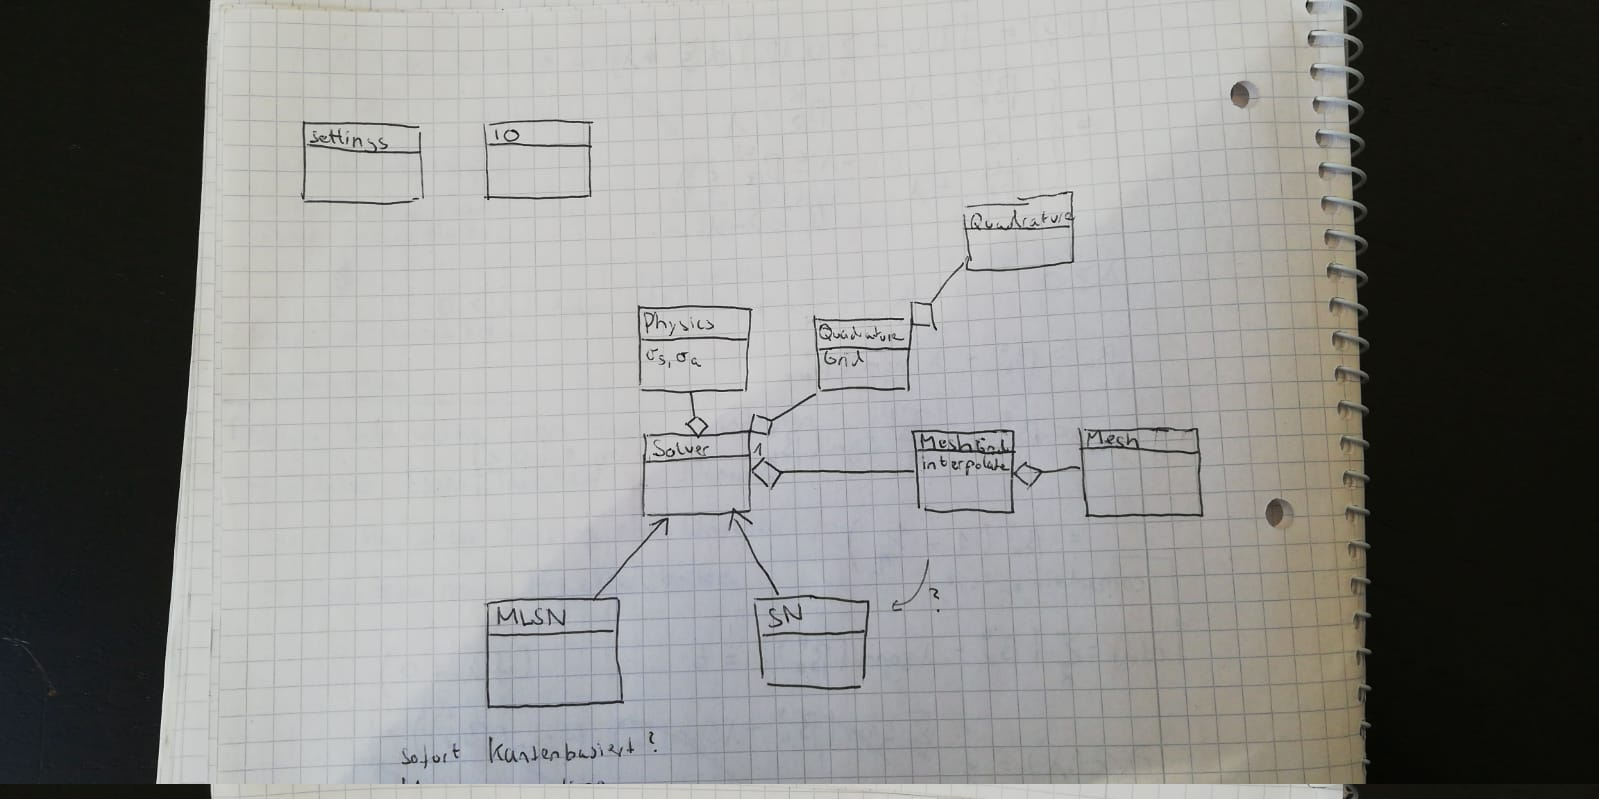
\includegraphics[scale=0.25]{test.jpeg}
\end{figure}
\newpage
\bibliographystyle{plain}  
\bibliography{references}

\end{document}
